%%%%%%%%%%%%%%%%%%%%%%%%%%%%%%%%%%%%%%%%%
% University Assignment Title Page 
% LaTeX Template
% Version 1.0 (27/12/12)
%
% This template has been downloaded from:
% http://www.LaTeXTemplates.com
%
% Original author:
% WikiBooks (http://en.wikibooks.org/wiki/LaTeX/Title_Creation)
%
% License:
% CC BY-NC-SA 3.0 (http://creativecommons.org/licenses/by-nc-sa/3.0/)
% 
% Instructions for using this template:
% This title page is capable of being compiled as is. This is not useful for 
% including it in another document. To do this, you have two options: 
%
% 1) Copy/paste everything between \begin{document} and \end{document} 
% starting at \begin{titlepage} and paste this into another LaTeX file where you 
% want your title page.
% OR
% 2) Remove everything outside the \begin{titlepage} and \end{titlepage} and 
% move this file to the same directory as the LaTeX file you wish to add it to. 
% Then add \input{./title_page_1.tex} to your LaTeX file where you want your
% title page.
%
%%%%%%%%%%%%%%%%%%%%%%%%%%%%%%%%%%%%%%%%%

%----------------------------------------------------------------------------------------
%	PACKAGES AND OTHER DOCUMENT CONFIGURATIONS
%----------------------------------------------------------------------------------------

\documentclass[12pt]{article}
\usepackage[utf8]{inputenc}
\usepackage[french]{babel}
\usepackage{bold-extra}
\usepackage{lmodern,textcomp}


%\usepackage{hyperref}

%% BIBTEX %%
\usepackage[backend=biber, sorting=none, style=numeric, natbib=true]{biblatex}
\DeclareCiteCommand{\supercite}[\mkbibsuperscript]
  {\iffieldundef{prenote}
     {}
     {\BibliographyWarning{Ignoring prenote argument}}%
   \iffieldundef{postnote}
     {}
     {\BibliographyWarning{Ignoring postnote argument}}}
  {\usebibmacro{citeindex}%
   \bibopenbracket\usebibmacro{cite}\bibclosebracket}
  {\supercitedelim}
  {}
\let\citep=\supercite
%\usepackage[round]{natbib}
%\addbibresource{Internet.bib}
%%

%% Centrer de grand tableau et figures %%
\usepackage{adjustbox}
\usepackage{array,multirow,makecell,tabularx}
\setcellgapes{1pt}
\makegapedcells
%\newcolumntype{R}[1]{>{\raggedleft\arraybackslash }b{#1}}
%\newcolumntype{L}[1]{>{\raggedright\arraybackslash }b{#1}}
%\newcolumntype{C}[1]{>{\centering\arraybackslash }b{#1}}
\newcolumntype{C}{>{\centering}X}
%%

\usepackage{longtable}
\usepackage{graphicx} 
\usepackage{xifthen}
\usepackage{tabularx}
\usepackage{adjustbox}
\usepackage{amsmath}
%\usepackage[clean,pdf]{svg}
\usepackage{pdfpages}
\usepackage[unicode,hidelinks]{hyperref}
\usepackage[]{url}
%\usepackage{tablefootnote}
\usepackage{footnote}
%\usepackage[bottom]{footmisc}
%\makesavenoteenv{tabular}
\makesavenoteenv{table}
\makesavenoteenv{tabularx}

%\usepackage[super,square]{natbib}

%\newenvironment{agrandirmarges}[2]{%
%\begin{list}{}{%
%\setlength{\topsep}{0pt}%
%\setlength{\listparindent}{\parindent}%
%\setlength{\itemindent}{\parindent}%
%\setlength{\parsep}{0pt plus 1pt}%
%\ifthenelse{\isodd{\value{page}}}%
%{\setlength{\leftmargin}{-#1}\setlength{\rightmargin}{-#2}}
%{\setlength{\leftmargin}{-#2}\setlength{\rightmargin}{-#1}}
%}\item }%
%{\end{list}}



%\usepackage[nottoc, notlof, notlot]{tocbibind}

\usepackage[left=4.2cm,right=4.2cm,top=3.5cm,bottom=3.5cm]{geometry}

\newcommand{\doctitle}{Proposition pour l'organisation du réseau}
\newcommand{\authorName}{Olivier \textsc{Radisson}}
\usepackage{fancyhdr}
\pagestyle{fancy}
\lhead{\doctitle}
\rhead{\authorName}
%\lfoot{Document réalisé par l'équipe n$^\circ$4}
\renewcommand{\headrulewidth}{0.4pt}
\renewcommand{\footrulewidth}{0.4pt}
\renewcommand{\newline}{~\\~\\}
\newcommand{\p}{\newline \indent}
\newcommand{\rt}{~\\ \indent}
\newcommand{\centergraph}[3][]{\begin{center}%
\begin{figure}[h!]%
\vspace{-5pt}%
\centerline{\includegraphics[width=#3]{#2}}%
\ifthenelse{\isempty{#1}}{}{\vspace{-8pt}\caption{#1}}%
\vspace{-5pt}%
\label{#2}%
\end{figure}%
\end{center}}
\newcommand{\newparagraph}{~\\\indent}

\setcounter{secnumdepth}{3}
%\setcounter{tocdepth}{2}


\begin{document}




\begin{titlepage}

\newcommand{\HRule}{\rule{\linewidth}{0.5mm}} % Defines a new command for the horizontal lines, change thickness here

\center % Center everything on the page
 
%----------------------------------------------------------------------------------------
%	HEADING SECTIONS
%----------------------------------------------------------------------------------------

\textsc{\LARGE Institut National des Sciences Appliquées de Lyon\\
\&\vspace{10pt}~
\\KompleXKapharnaüM}\\[1.0cm] % Name of your university/college
\textsc{\small Stage de 4\up{ème} année du département Génie Électrique} \\[0.2cm]
\textsc{\Large Projet Do Not Clean}
\\[0.5cm] % Major heading such as course name
\textsc{\large Réalisation d'une carte multimédia programmable et contrôlable via wifi}\\[0.5cm] % Minor heading such as course title

%----------------------------------------------------------------------------------------
%	TITLE SECTION
%----------------------------------------------------------------------------------------

\HRule \\[0.4cm]
%{ \huge  \textsc{\textbf{Plan Projet}}}\\[0.4cm] % Title of your document
{ \huge   \scshape{\doctitle}  } % \bfseries
\HRule \\[1.5cm]
 
%----------------------------------------------------------------------------------------
%	AUTHOR SECTION
%----------------------------------------------------------------------------------------

\begin{minipage}{0.4\textwidth}
\begin{flushleft} \large
\emph{Auteur:}\\
Olivier \textsc{Radisson}\\
~ \\
~ \\
~ \\
~ \\
\end{flushleft}
\end{minipage}
~
\begin{minipage}{0.4\textwidth}
\begin{flushright} \large
\emph{Tuteur de stage :} \\
Gilles \textsc{Gallet}
~ \\
~ \\
\emph{Chef de projet :} \\
Pierre \textsc{Hoezelle}
~ \\
~ \\

\end{flushright}
\end{minipage}\\[2cm]

% If you don't want a supervisor, uncomment the two lines below and remove the section above
%\Large \emph{Author:}\\
%John \textsc{Smith}\\[3cm] % Your name

%----------------------------------------------------------------------------------------
%	DATE SECTION
%----------------------------------------------------------------------------------------
\vspace{2.2cm}
{\large - 6 octobre 2014 -}\\ \vspace{10pt}
{\large Dernière édition le \today}\\
%{\large  ~~~ : \today}\\[3cm] % Date, change the \today to a set date if you want to be precise

%----------------------------------------------------------------------------------------
%	LOGO SECTION
%----------------------------------------------------------------------------------------

%\includegraphics{Logo}\\[1cm] % Include a department/university logo - this will require the graphicx package
 
%----------------------------------------------------------------------------------------

\vfill % Fill the rest of the page with whitespace

\end{titlepage}


%\newpage
%~
%	\thispagestyle{empty}
    

\newpage
\thispagestyle{empty}
\begin{abstract}
Ce document présente une proposition pour l'organisation du réseau.\\
Il est prévu de pouvoir déployer un grand nombre de carte, d'une dizaine a plusieurs centaines si besoin, et de les faire communiquer ensemble dans un même réseau. Comme tout réseau, il y a besoin de prévoir des régles de communication et c'est de cela qu'il est question dans ce document.\\
Seront donc abordé les thèmes suivant:
\begin{itemize}
\item Hiérarchie et connaissance du réseau
\item Protocols de communication
\item Protocols de transport de l'information
\item Groupes de cartes et multi-casting
\end{itemize}

\end{abstract}

\newpage
~ \thispagestyle{empty}
%\newpage
%\thispagestyle{empty}

\tableofcontents

%\newpage
%~ \thispagestyle{empty}
\newpage

\setcounter{page}{1}

\section{Introduction}
\textit{Ce document à une visée majoritairement technique. En revanche il est question de l'organisation du réseau et la communication des cartes entre elles, il y a donc un certain nombre de points qui peuvent être intéressants pour les utilisateurs}\p
Les cartes seront toutes membre d'un réseau, certaines même feront le pont entre un réseau wifi et un réseau radio. Pour le bon fonctionnement de celui-ci nous allons voir comment organiser celui-ci en définissant un certain nombre de règles.\p
Ce document présente une première proposition fruit d'une réflexion en amont et des contraintes qui ont été soulevé par la première proposition du système de scénario. Cette proposition nait également d'un retour sur connaissance du système qui avait été mit en place pour figures libres.

\section{Présentation du réseau}
Le réseau est composé d'un réseau principal en WIFI et de sous réseaux annexes en liaison radio. La jonction entre les deux se fera via des cartes possédant une interface WIFI et une interface radio. Ces cartes auront pour vocation de contrôler l'ensemble de leur sous réseau radio.\p
Au sein du réseau vivent un certains nombre de périphériques distincts dont voici la liste: 
\begin{itemize}
\item Des cartes WIFI
\item Des télécommandes WIFI
\item Des régies WIFI
\item Des cartes WIFI et Radio
\item Des cartes Radio
\item Des périphériques OSC
\item Des routeurs WIFI
\end{itemize}~\\
\indent Chaque entité pourra appartenir à des groupes dont certains seront conseillé notamment :
\begin{itemize}
\item Groupe actionneur
\item Groupe télécommande
\item Groupe régie
\item Groupe gateway
\end{itemize}~\\ \indent
Cette liste n'est pas exhaustive mais présente des groupes qui seront assez présent. Il sera possible de rajouter autant de groupe que voulu, chaque périphérique devra seulement stipulé qu'il fait parti de tel et tel groupes.\p
Ce graphique résume l'organisation du réseau :

\begin{figure}[htbp]
  \centering
  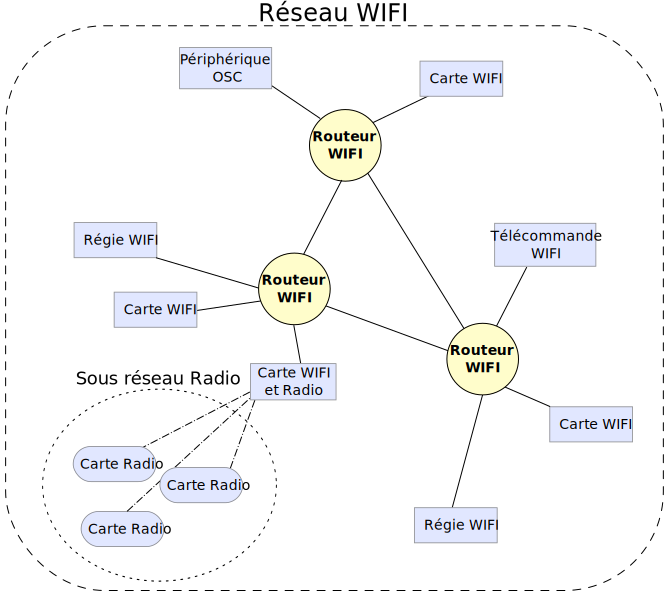
\includegraphics[width=0.85\textwidth]{figs/structure_reseau_global.pdf}
  \caption{Structure globale du réseau}
  \label{fig:structure_globale}
  %\vspace{-17pt}
\end{figure}

\subsection{Éléments du réseau}
Les différents élements du réseau sont détaillé ci-dessous.

\paragraph{Cartes WIFI}\p
Les cartes WIFI sont tous les éléments qui sont basés sur la carte que nous allons créer et qui sont vouez à être des actionneurs.
\paragraph{Télécommandes WIFI}\p
Les télécommandes WIFI sont des cartes WIFI qui n'ont pas vocation à avoir de sorties autre que WIFI et ont en revanche un ensemble de boutons d'entrées pour déclencher des signaux sur le réseau. Ce sont les IHM embarqués du réseau.
\paragraph{Régies WIFI}\p
Les régies WIFI sont des périphériques qui font tourner le logiciel de régie. Ils n'ont pas vocation à être des actionneurs, mais possède le moyen d'envoyer des ordres sur le réseau mais aussi d'afficher des informations tel que l'état des cartes.
\paragraph{Cartes WIFI et Radio}\p
Les cartes WIFI et Radio sont simplement des cartes similaire aux précédentes mais qui possèdent en plus une interface Radio pour pouvoir piloter un sous réseau radio. Ces cartes sont celles qui joueront le scénario pour l'ensemble du sous réseau.
\paragraph{Cartes Radio}\p
Les cartes Radio sont des cartes qui ne possède pas le Yun Shield et donc pas d'interface réseau. Sans Yun Shield les cartes n'ont donc pas de processeur Dragino non plus, et ne peuvent donc pas jouer de scénario. Ils recevront donc juste des ordres de la part des cartes WIFI et Radio.
\paragraph{Périphériques OSC}\p
Ces périphériques désignent tous les éléments qui n'ont pas été conçu par nous mais qui sont capable d'émettre des ordres WIFI tel par exemple un smartphone avec TouchOSC.
\paragraph{Routeurs WIFI}\p
Les routeurs wifi sont les points de relais entre les différents autres éléments du réseau pour palier à la faible porter du WIFI.

\subsection{Protocoles envisagés}

Les protocoles de communication sont des éléments important et structurels du réseau, il est important de les choisir avec précaution. Nous allons dans un premier temps lister les protocoles qui seront surement utilisé dans le réseau.

\subsubsection{Protocoles de liaison (niveau 2)}
Deux protocoles seront utilisés conjointement pour la couche de liaison.
\paragraph{WIFI}\rt Le protocole WIFI sera utilisé dans la majeure partie du temps. Il servira comme réseau de base entre les différents éléments de celui-ci.
\paragraph{Radio}\rt Un protocole Radio sera utilisé par les interfaces Radio pour communiquer avec la carte WIFI qui servira de gateway à l'ensemble d'un sous-réseau.

\subsubsection{Protocole de réseau (niveau 3)}
\paragraph{IP}\rt Le protocole IP est un protocole de base de la couche réseau, il sera massivement utilisé pour transmettre les messages entre les périphériques du réseau.
\paragraph{DHCP}\rt Le protocole DHCP pourra être utilisé pour l'allocation dynamique des adresse IP.
\paragraph{ARP}\rt Le protocole ARP sera présent pour la résolution entre l'adresse IP et l'adresse MAC des éléments du réseau. C'est un protocole qui sera géré par le système d'exploitation et non par notre système.

\subsubsection{Protocole de transport (niveau 4)}
Les deux protocoles majeurs de transport seront utilisés
\paragraph{TCP}\rt Le protocole TCP sera utilisé pour les ordres important tels que le déclenchement de plusieurs sources simultanées, et pour l'organisation du réseau.
\paragraph{UDP}\rt Le protocole UDP sera utilisé pour les ordres demandant une faible latance et n'étant pas critique. Il servira également pour la compatibilité avec la majeure partie des équipement OSC déjà existant.

\subsubsection{Protocole applicatif (niveau 7)}
\paragraph{OSC}\rt Le protocole OSC sera le protocole haut niveau de référence pour l'échange d'information sur le réseau.
\paragraph{SSH}\rt Pour certaines actions critiques, notamment si le système plante, le protocole SSH permettra un accès directe aux cartes WIFI pour les faire redémarrer.
\paragraph{FTP}\rt Le protocoles FTP sera surement celui choisit pour le transfert de média entre la régie et les cartes.

\section{Organisation du réseau}

\subsection{Identification sur le réseau}
Chaque élément du réseau sera représenté par les informations suivantes :
\begin{table}[htbp]
\centering
\begin{adjustbox}{center}
\small
\begin{tabularx}{\textwidth}{|c|C|c|C|c|}
\hline
\textbf{Nom unique} & \textbf{IP} & \textbf{Port} & \textbf{Groupes} & \textbf{Prêt} \tabularnewline
\hline
\hline
Titreur\_1 & 192.168.0.10 & 3028 & actionneur~:~titreur & True \tabularnewline
\hline
Titreur\_2 & 192.168.0.11 & 3028 & actionneur~:~titreur & True \tabularnewline
\hline
Poubelle\_angle & 192.168.0.14 & 3028 & actionneur & False \tabularnewline
\hline
\end{tabularx}
\normalsize
\end{adjustbox}
\label{tab:ARP table example}
\caption{Exemple de représentation}
\end{table}~\\
Ces informations seront retenues par l'ensemble des éléments du réseau et serviront pour que ceux-ci puissent communiquer entre eux.

\subsection{Hiérarchie dans le réseau}
Il ne devrait y avoir aucune hiérarchie à l'intérieur du réseau et chaque périphérique pourra s'adresser à un autre qui lui répondra sans distinction. Ce choix est motivé principalement parce qu'il n'y a pas d'intérêt apparent à la mise en place d'une hiérarchie d'autant que nous contrôlerons tous les éléments du réseau, et que garder cette souplesse peut permettre des comportements intéressants.\p
Seul un élément sera distingué des autres, le plus vieux membre du réseau aura un statu un petit peu particulier.

\subsection{Inscription sur le réseau WIFI}
L'inscription sur le réseau se ferra tout d'abord par la connexion à l'une des antennes WIFI. Je pense que l'attribution dynamique d'une adresse IP n'est pas une mauvaise chose et qu'au contraire, vu que les cartes en seront capable, cela permettra une plus grande souplesse dans le réseau.\p
Une fois connecté chaque élément va se présenter au réseau pour que le restes des membres puisse le rajouter dans une table permettant que chaque nœud ait une connaissance globale du réseau. Pour que le nouveau venu ait la même connaissance un élément du réseau va lui envoyer une copie de sa table pour qu'il n'y ait pas besoin que chaque nœud réinforme l'ensemble du réseau de sa présence.

\subsubsection{Attribution d'une adresse IP}
Pour se voir obtenir une adresse IP, l'élément du réseau va tout d'abord faire une demande DHCP à la passerelle du réseau pour qu'elle lui en octroie une.

\subsubsection{Présentation sur le réseau}
Pour se présenter sur le réseau le nouveau venu va émettre un message sur l'adresse de broadcast du réseau et sur un port fixé à l'avance. Ce port ne pourra pas être alloué dynamiquement et ce devra donc être une constante du réseau.\p
La première trame aura cette forme : ~\\

\begin{table}[htbp]
\centering
{
\textbf{Trame OSC}\vspace{8pt}~\\
\begin{tabularx}{0.85\textwidth}{|c|c|c|C|}
\hline
\textbf{IP} & \textbf{Port} & \textbf{Protocole} & \textbf{Adresse}  \tabularnewline
\hline
\hline
X.X.X.255 & 3000 & TCP & /protocol/newhere \tabularnewline
\hline
\end{tabularx}
\vspace{10pt}
~\\\textbf{Arguments}\vspace{5pt}\\
}
\begin{adjustbox}{center}
\small
\begin{tabularx}{0.6\textwidth}{|c||c|C|}
\hline
\textbf{Champs} & \textbf{Type} & \textbf{Valeur}  \tabularnewline
\hline
\hline
Nom & string & Titreur  \tabularnewline
\hline
Port & int & 3028  \tabularnewline
\hline
Groupes & string & actionneur~:~titreur \tabularnewline
\hline
Prêt & bool & False  \tabularnewline
\hline
\end{tabularx}
\normalsize
\end{adjustbox}
\label{tab:trame_newhere}
\caption{Exemple de trame \textsl{/protocol/newhere}}
\vspace{-25pt}
\end{table}~\p
Elle sera reçus par tous les membres du réseau qui mettrons à jour leur carte du réseau en y ajoutant le dernier venu.\p
Que se passe t-il si un membre du réseau possède déjà le même nom que celui de dernier arrivant ? Il y a conflit et celui-ci doit être réglé pour éviter les comportements chaotiques. Pour cela le réseau va exclure le nouveau en lui stipulant ainsi :


\begin{table}[htbp]
\centering

\textbf{Trame OSC}\vspace{8pt}~\\

\begin{tabularx}{0.85\textwidth}{|c|c|c|C|}
\hline
\textbf{IP} & \textbf{Port} & \textbf{Protocole} & \textbf{Adresse}  \tabularnewline
\hline
\hline
X.X.X.X\footnotemark[1] & PPPP\footnotemark[2] & TCP & /protocol/conflict \tabularnewline
\hline
\end{tabularx}
\vspace{10pt} 
%~\\\textbf{Arguments}\vspace{5pt}\\
%}
%\begin{adjustbox}{center}
%\small
%\begin{tabularx}{0.6\textwidth}{|c||c|C|}
%\hline
%\textbf{Champs} & \textbf{Type} & \textbf{Valeur}  \tabularnewline
%\hline
%\hline
%Nom & string & Titreur  \tabularnewline
%\hline
%Port & int & 3028  \tabularnewline
%\hline
%Groupes & string & actionneur~:~titreur \tabularnewline
%\hline
%Prêt & bool & False  \tabularnewline
%\hline
%\end{tabularx}
%\normalsize
%\end{adjustbox}
\label{tab:trame_newhere}
\caption{Trame \textsl{/protocol/conflict}}
\vspace{-25pt}
\end{table}
\footnotetext[1]{IP du nouvel arrivant}
\footnotetext[2]{Port du nouvel arrivant}
~\p
Dans le cas ou le nom du nouvel arrivant est bien unique sur le réseau, le parent du réseau va lui envoyer la liste des autres nœud du réseau un a un via une trame OSC puis il indiquera qu'il a finit de décrire le réseau en émettant une trame OSC finale.
\newpage
\begin{table}[htbp]
\centering
{
\textbf{Trame OSC}\vspace{8pt}~\\
\begin{tabularx}{0.85\textwidth}{|c|c|c|C|}
\hline
\textbf{IP} & \textbf{Port} & \textbf{Protocole} & \textbf{Adresse}  \tabularnewline
\hline
\hline
X.X.X.X & PPPP & TCP & /protocol/netmap/node \tabularnewline
\hline
\end{tabularx}
\vspace{10pt}
~\\\textbf{Arguments}\vspace{5pt}\\
}
\begin{adjustbox}{center}
\small
\begin{tabularx}{0.6\textwidth}{|c||c|C|}
\hline
\textbf{Champs} & \textbf{Type} & \textbf{Valeur}  \tabularnewline
\hline
\hline
IP & string &X.X.X.30  \tabularnewline
\hline
Nom & string & Poubelle\_Son  \tabularnewline
\hline
Port & int & 3028  \tabularnewline
\hline
Groupes & string & actionneur \tabularnewline
\hline
Prêt & bool & True  \tabularnewline
\hline
\end{tabularx}
\normalsize
\end{adjustbox}
\label{tab:trame_newhere}
\caption{Exemple de trame \textsl{/protocol/netmap/node}}
\vspace{-25pt}
\end{table}~\p
La trame de fin ressemblera à ceci :
\begin{table}[htbp]
\centering

\textbf{Trame OSC}\vspace{8pt}~\\

\begin{tabularx}{0.85\textwidth}{|c|c|c|C|}
\hline
\textbf{IP} & \textbf{Port} & \textbf{Protocole} & \textbf{Adresse}  \tabularnewline
\hline
\hline
X.X.X.X\footnotemark[1] & PPPP\footnotemark[2] & TCP & /protocol/netmap/end \tabularnewline
\hline
\end{tabularx}
\vspace{10pt} 
%~\\\textbf{Arguments}\vspace{5pt}\\
%}
%\begin{adjustbox}{center}
%\small
%\begin{tabularx}{0.6\textwidth}{|c||c|C|}
%\hline
%\textbf{Champs} & \textbf{Type} & \textbf{Valeur}  \tabularnewline
%\hline
%\hline
%Nom & string & Titreur  \tabularnewline
%\hline
%Port & int & 3028  \tabularnewline
%\hline
%Groupes & string & actionneur~:~titreur \tabularnewline
%\hline
%Prêt & bool & False  \tabularnewline
%\hline
%\end{tabularx}
%\normalsize
%\end{adjustbox}
\label{tab:trame_newhere}
\caption{Trame \textsl{/protocol/netmap/end}}
\vspace{-25pt}
\end{table}\p


   
   



\end{document}